\documentclass[10pt,a4paper]{article}
\usepackage[UTF8,fontset = windows]{ctex}
\setCJKmainfont[BoldFont=黑体,ItalicFont=楷体]{华文中宋}
\usepackage{amssymb,amsmath,amsfonts,amsthm,mathrsfs,dsfont,graphicx}
\usepackage{ifthen,indentfirst,enumerate,color,titletoc}
\usepackage{tikz}
\usepackage{multicol}
\usepackage{makecell}
\usepackage{longtable}
\usetikzlibrary{arrows,calc,intersections,patterns,decorations.pathreplacing,3d,angles,quotes}
\usepackage[bf,small,indentafter,pagestyles]{titlesec}
\usepackage[top=1in, bottom=1in,left=0.8in,right=0.8in]{geometry}
\renewcommand{\baselinestretch}{1.65}
\newtheorem{defi}{定义~}
\newtheorem{eg}{例~}
\newtheorem{ex}{~}
\newtheorem{rem}{注~}
\newtheorem{thm}{定理~}
\newtheorem{coro}{推论~}
\newtheorem{axiom}{公理~}
\newtheorem{prop}{性质~}
\newcommand{\blank}[1]{\underline{\hbox to #1pt{}}}
\newcommand{\bracket}[1]{(\hbox to #1pt{})}
\newcommand{\onech}[4]{\par\begin{tabular}{p{.9\textwidth}}
A.~#1\\
B.~#2\\
C.~#3\\
D.~#4
\end{tabular}}
\newcommand{\twoch}[4]{\par\begin{tabular}{p{.46\textwidth}p{.46\textwidth}}
A.~#1& B.~#2\\
C.~#3& D.~#4
\end{tabular}}
\newcommand{\vartwoch}[4]{\par\begin{tabular}{p{.46\textwidth}p{.46\textwidth}}
(1)~#1& (2)~#2\\
(3)~#3& (4)~#4
\end{tabular}}
\newcommand{\fourch}[4]{\par\begin{tabular}{p{.23\textwidth}p{.23\textwidth}p{.23\textwidth}p{.23\textwidth}}
A.~#1 &B.~#2& C.~#3& D.~#4
\end{tabular}}
\newcommand{\varfourch}[4]{\par\begin{tabular}{p{.23\textwidth}p{.23\textwidth}p{.23\textwidth}p{.23\textwidth}}
(1)~#1 &(2)~#2& (3)~#3& (4)~#4
\end{tabular}}
\begin{document}
\begin{enumerate}[1.]



\item 写出下列直线的一个方向向量$\overrightarrow d$.\\
(1) $2x-3y+1=0$;\\ 
(2) $3x+1=0$;\\
(3) $4-2y=0$.
\item 求过点$P$且与$\overrightarrow d$平行的直线$l$的点方向式方程.\\
(1) $P(0,0)$, $\overrightarrow d=(1,1)$;\\
(2) $P(-2,3)$, $\overrightarrow d=(-2,3)$.
\item 求经过$AB$两点的直线$l$的点方向式方程.\\
(1) $A(3,5)$, $B(1,0)$;\\ 
(2) $A(2,2)$, $B(5,5)$.
\item 已知平行四边形$ABCD$的三个顶点的坐标分别为$A(1,2)$、$B(3,4)$、$C(2,6)$, 求四条边$AB,BC,CD$和$DA$所在直线的点方向式方程.
\item 求下列直线的一个法向量$\overrightarrow n$.\\
(1) $2x-3y+1=0$;\\
(2) $\dfrac x2+\dfrac y5=1$.
\item 求经过点$P$且垂直于向量$\overrightarrow n$的直线的点法向式方程.\\
(1) $P(0,0)$, $\overrightarrow n=(1,1)$;\\
(2) $P(5,2)$, $\overrightarrow n=(0,2)$.
\item 已知直线$\dfrac{x-2}3=\dfrac{y+1}2$的一个法向量为$\overrightarrow n=(a,a-2)$, 求实数$a$的值.
\item 已知$\triangle ABC$的三个顶点的坐标分别为$A(3,8)$、$B(3,-2)$、$C(-3,0)$.\\
(1) 求$BC$边所在直线的方程;\\
(2) 求$AB$边上中线$CM$所在直线的方程;\\
(3) 求$BC$边上高$AD$所在直线的方程.
\item 已知四边形$ABCD$是平行四边形, $AB$边所在直线的方程是$x+y-1=0$, $AD$边所在直线的方程是$3x-y+4=0$, 顶点$C$的坐标是$(3,3)$, 求这个平行四边形其他两条边所在直线的方程.
\item 已知$\triangle ABC$的两个顶点的坐标分别是$A(-2,1)$、$B(4,-3)$, 且$\triangle ABC$的垂心坐标为$H(0,2)$, 分别求$BC,AC$边所在直线的方程.
\item 已知$\triangle ABC$的三个顶点的坐标分别为$A(2,1)$、$B(0,7)$、$C(-4,-1)$.\\
(1) 求此三角形的三边所在直线的方程;\\
(2) 求此三角形的三条中线所在直线的方程.
\item 已知$\triangle ABC$的三个顶点的坐标分别$A(4,0)$、$B(6,7)$、$C(0,3)$, 求此三角形的三条高所在直线的方程.
\item 已知梯形$ABCD$的三个顶点的坐标分别为$A(2,3)$、$B(-2,1)$、$C(4,5)$, 求此梯形中位线所在直线的方程.
\item 已知$A(1,-1)$、$B(3,3)$两点, 点$C(5,a)$在直线$AB$上, 求实数$a$的值.
\item 填空:
方程$\begin{vmatrix} x+1 & y-1  \\4 & 1  \end{vmatrix}=0$所表示的直线的一个法向量是\blank{50}.
\item 已知原点$O$在直线$l$上的射影为$H(-2,1)$, 求直线$l$的方程.
\item 已知$A(7,-4)$、$B(-5,6)$两点, 求线段$AB$的垂直平分线的方程.
\item 已知$\triangle ABC$的两个顶点的坐标分别是$A(2,2)$、$B(3,0)$, 此三角形的重心坐标为$(3,1)$.\\
(1) 求此三角形的三边所在直线的方程;\\
(2) 求此三角形的三条中线所在直线的方程.
\item 已知$a,b,c$是互不相等的正实数, 求经过下列两点的直线的倾斜角:\\
(1) $A(a,c),B(b,c)$;\\
(2) $C(a,\sqrt {a^2+b^2}),D(a,\sqrt {b^2+c^2})$;\\
(3) $E(b,b+c),F(a,a+c)$;\\
(4) $G(b,a^2),H(a,b^2)$.
\item 已知斜率为$3$的直线过点$(1,1)$和$(x,-2)$, 求实数$x$的值.
\item 求下列方程所表示的直线的斜率:\\
(1) $x+5=0$;\\
(2) $2y+3=0$;\\
(3) $\dfrac{x-3}3=\dfrac{y+1}{-4}$;\\
(4) $5x+6y+3=0$.
\item 已知直线$l$的倾斜角为$\alpha$, 且这条直线经过点$P(3,5)$, 求直线$l$的方程.\\
(1) $\alpha =\dfrac{\pi }4$;\\ 
(2) $\alpha =0$;\\
(3) $\alpha =\dfrac{\pi}2$.
\item 写出经过下列两点的直线的点斜式方程.\\
(1) $A(-3,0),B(2,-2)$;\\ 
(2) $P(2,-2),Q(0,1)$.
\item 求过点$(\sqrt 3,\sqrt 5)$, 倾斜角等于直线$y=\sqrt 3x+1$的倾斜角的一半的直线方程.
\item 已知直线$l$的倾斜角为$\alpha$, $\sin \alpha =\dfrac 35$, 且这条直线经过点$P(3,5)$, 求直线$l$的一般式方程.
\item 已知矩形$OACB$的顶点的坐标分别为$O(0,0)$、$A(8,0)$、$B(0,5)$, 求该矩形的对角线所在直线的方程.
\item 已知直线$2x-3y+6=0$, 这条直线的点方向式方程可以是\bracket{20}.
\fourch{$\dfrac{x-3}2=\dfrac{y-4}3$}{$\dfrac x{-2}=\dfrac{y-2}3$}{$\dfrac{x+3}3=\dfrac y2$}{$\dfrac{x+3}2=\dfrac y3$}
\item 求过点$P$且平行于直线$l_0$的直线的一般式方程.\\
(1) $P(2,1)$, $l_0:x+4=0$;\\ 
(2) $P(1,2)$, $l_0:\dfrac x3+\dfrac y4+\dfrac 17=0$.
\item 求过点$P$且垂直于直线$l_0$的直线的一般式方程.\\
(1) $P(2,1)$, $l_0:y-3=0$;\\ 
(2) $P(-2,-1)$, $l_0:\dfrac{x-1}3=\dfrac{y+2}4$.
\item 分别根据下列条件, 求相应直线$l$的方程.\\
(1) 直线$l$经过$A(2,0)$、$B(3,7)$两点;\\
(2) 直线$l$经过点$P(3,4)$, 且与向量$\overrightarrow d=(1,-1)$平行;\\
(3) 直线$l$与$x$轴交于点$A(3,0)$, 与$y$轴交于点$B(0,-1)$;\\
(4) 直线$l$经过点$P(3,2)$, 且与向量$\overrightarrow n=(8,-4)$垂直.
\item 选择题:
直线$x-ay+2=0(a<0)$的倾斜角是\bracket{20}.
\fourch{$\arctan \dfrac 1a$}{$-\arctan \dfrac 1a$}{$\pi -\arctan \dfrac 1a$}{$\pi +\arctan \dfrac 1a$}
\item 当$\theta \in [-\dfrac{\pi }2,0)$时, 求经过$P(0,0)$、$Q(\cos \theta ,\sin \theta)$两点的直线的斜率.
\item 已知$\triangle ABC$的顶点坐标分别为$A(-3,0)$、$B(1,2)$、$C(3,9)$, 直线$l$过顶点$C$, 且把$\triangle ABC$分为面积相等的两部分, 求直线$l$的方程.
\item 已知直线$l$经过点$A(3,4)$, 它的倾斜角是直线$2x-y+1=0$的倾斜角的$2$倍, 求直线$l$的方程.
\item 一个弹簧在挂$4$千克的物体时, 长$20$厘米, 在弹性限度内, 所挂物体的重量每增加$1$千克, 弹簧伸长$1.5$厘米.写出弹簧的长度$y$(厘米)与所挂物体重量$x$(千克)之间关系的方程.
\item 一根金属棒在$30^\circ\text{C}$时长$14.205$米, 在$60^\circ\text{C}$时长$14.211$米.已知长度$y$(米)和温度$x$($^\circ\text{C}$)的关系可以用直线方程来表示, 试写出这条直线的方程, 并求$80^\circ\text{C}$时这根金属棒的长度.
\item 判断下列各组直线的位置关系:\\
(1) $l_1$: $2x-3y-1=0$, $l_2$: $4x-6y-2=0$;\\
(2) $l_1$: $\dfrac x3-\dfrac{12}5y+1=0$, $l_2$: $36x+5y-1=0$;\\
(3) $l_1$: $y=\dfrac 13(x-6)$, $l_2$: $3x+y-3=0$;\\
(4) $l_1$: $(\sqrt 5+1)x-2y+1=0$, $l_2$: $2x-(\sqrt 5-1)y-1=0$.
\item 已知直线$l_1$: $6x+(t-1)y-8=0$与直线$l_2$: $(t+4)x+(t+6)y-16=0$.\\
(1) 当$t$为何值时, $l_1$与$l_2$相交?\\
(2) 当$t$为何值时, $l_1$与$l_2$平行?\\
(3) 当$t$为何值时, $l_1$与$l_2$重合?\\
(4) 当$t$为何值时, $l_1$与$l_2$垂直?
\item 已知直线$l_1$: $mx+8y+n=0$与直线$l_2$: $2x+my-1=0$.当直线$l_1$与直线$l_2$分别满足下列条件时, 求实数$mn$的值.\\
(1) 直线$l_1$与直线$l_2$平行;\\
(2) 直线$l_1$与直线$l_2$垂直, 且直线$l_1$在$y$轴上的截距为$-1$.
\item 根据下列条件, 写出满足条件的直线的一般式方程.\\
(1) 经过直线$2x-y+1=0$与直线$2x+2y-1=0$的交点, 且与直线$5x-y=0$垂直;\\
(2) 经过直线$x-y+1=0$与直线$2x-y+2=0$的交点, 且与直线$3x+4y=12$平行.
\item 已知直线$l_1$: $y=kx+k+2$与直线$l_2$: $y=-2x+4$的交点在第一象限, 求实数$k$的范围.
\item 已知集合$A=\{(x,y)|x-y-1=0,\ x,y\in \mathbf{R}\}$, 集合$B=\{(x,y)|ax-y+2=0,\ x,y\in \mathbf{R}\}$, 且$A\cap B=\varnothing$, 求实数$a$的值.
\item 是否存在实数$a$, 使直线$l_1$: $(a-1)x+(a-2)y-1=0$与直线$l_2$: $6x+(2a-3)y-3=0$平行? 若存在, 求$a$的值; 若不存在, 请说明理由.
\item 若直线$mx-2y=1$与直线$6x-4y+n=0$重合, 求实数$m,n$的值.
\item 若直线$(2a^2-7a+3)x+(a^2-9)y+3=0$与$x$轴平行, 求实数$a$的值.
\item 求下列两组直线的夹角:\\
(1) $l_1$: $\sqrt 3x-y=0$, $l_2$: $x-\sqrt 3y+2=0$;\\
(2) $l_1$: $x-1=0$, $l_2$: $x+y-5=0$.
\item 已知直线$\sqrt 3x+y=0$与直线$kx-y+1=0$的夹角为$60^{\circ }$, 求实数$k$的值.
\item 已知等腰直角三角形$ABC$的斜边$AB$所在直线的方程为$3x-y-5=0$, 直角顶点为$C(4,-1)$, 求两条直角边所在直线的方程.
\item 判断直线$l_1$与直线$l_2$的位置关系.\\
(1) $l_1$: $2x-3=0$, $l_2$: $ax+y-1=0$, 其中$a\in \mathbf{R}$;\\
(2) $l_1$: $(a^2+1)x+y-1=0$, $l_2$: $(2a^2+3)x+y+a=0$, 其中$a\in \mathbf{R}$.
\item 已知直线$y=ax+b$的倾斜角为$\dfrac{3\pi }4$, 且这条直线与直线$5x+3y-31=0$的交点在第一象限内, 求实数$b$的取值范围.
\item 已知直线$l_1$: $ax+by+4=0$, 直线$l_2$: $(1-a)x-y-b=0$, 直线$l_3$: $x+2y+3=0$, 且这三条直线两两平行, 求实数$ab$的值.
\item 已知等腰直角三角形$ABC$的直角边$BC$所在直线的方程为: $x-2y-6=0$, 顶点$A$的坐标为$(0,6)$, 求斜边$AB$和直角边$AC$所在直线的方程.
\item 已知直线$l_1$: $a_1x+b_1y+c_1=0$(实数$a_1,b_1$不同时为零), 直线$l_2$: $a_2x+b_2y+c_2=0$(实数$a_2,b_2$不同时为零), 用$l_1$与$l_2$的法向量求这两条直线的夹角.
\item 求点$P(3,2)$到直线$l$: $3x-2y=13$的距离.
\item 已知$P(0,0)$、$Q(3,2)$两点, 试判断$P,Q$是否在下列直线的同一侧.\\
(1) $2x+3y=4$;\\ 
(2) $x+3y+4=0$;\\
(3) $2x-3y=4$;\\ 
(4) $-2x-3y+3=0$.
\item 已知直线$l_1$: $2x-y+a=0$与直线$l_2$: $-4x+2y+1=0$, 且直线$l_1$与直线$l_2$的距离为$\dfrac{7\sqrt 5}{10}$, 求实数$a$的值.
\item 已知点$P$为直线$3x-4y+2=0$上的任意一个动点, 求点$P$到点$A(3,-1)$的距离的最小值.
\item 已知$A(2,3)$、$B(-4,8)$两点, 直线$l$经过原点, 且$AB$两点到直线$l$的距离相等, 求直线$l$的方程.
\item 已知平行直线$l_1$与$l_2$的距离为$\sqrt 5$, 且直线$l_1$经过原点, 直线$l_2$经过点$(1,3)$, 求直线$l_1$和直线$l_2$的方程.
\item 已知直线$l$过点$P(0,1)$, 且被平行直线$l_1$: $3x+4y-8=0$与$l_2$: $3x+4y+2=0$所截得的线段的长为$2\sqrt 2$, 求直线$l$的方程.
\item 求与直线$x-2y+1=0$和$2x-y+3=0$距离相等的点的轨迹.
\item 已知正方形$ABCD$的中心的坐标为点$P(1,1)$, $AB$边所在直线的方程为$x+2y+3=0$.求这个正方形的其他三边所在直线的方程.
\item 求原点$O$到直线$x\cos \theta +y\sin \theta +2=0$, $\theta \in \mathbf{R}$的距离.
\item 已知直线$l$过点$(2,4)$, 且它被平行直线$l_1$: $x-y+1=0$与直线$l_2$: $x-y-2=0$所截得的线段的中点在直线$l_3$: $x+2y-3=0$上, 求直线$l$的方程.
\item 已知$P_1(1,0)$、$P_{2}(7,-8)$两点分别在直线$l$的两侧, 且$P_1,P_2$到直线$l$的距离均为$4$, 求直线$l$的方程.
\item 若直线$l$过点$P(0,2)$, 它的一个方向向量为$(1,1)$, 则直线$l$的方程是\blank{50}.
\item 若直线$l$过点$(3,1)$, 且$l$的法向量$\overrightarrow n=(1,3)$, 则直线$l$的方程为\blank{50}.
\item 经过点$P(x_0,y_0)$, 且与向量$\overrightarrow d=(u,v)$平行的直线方程是\bracket{20}.
\fourch{$\dfrac{x-x_0}u=\dfrac{y-y_0}v$}{$\dfrac{x-{x_0}}{y-{y_0}}=\dfrac uv$}{$y-y_0=\dfrac vu(x-x_0)$}{$u(y-y_0)=v(x-x_0)$}
\item 若直线$x=1$的倾斜角为$\theta$, 则$\theta$等于\bracket{20}.
\fourch{$0$}{$\dfrac{\pi }4$}{$\dfrac{\pi }2$}{不存在}
\item 如图, 已知矩形$OABC$的顶点$A$的坐标为$(5,2)$, 求直线$AB$的方程.
\begin{center}
    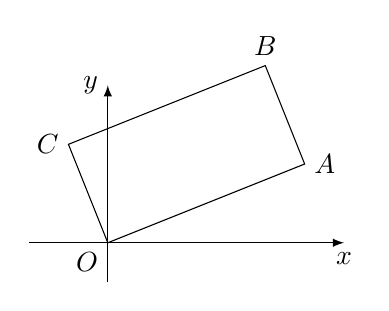
\begin{tikzpicture}[>=latex, scale = 0.5]
        \draw [->] (-2,0) -- (6,0) node [below] {$x$};
        \draw [->] (0,-1) -- (0,4) node [left] {$y$};
        \draw (0,0) node [below left] {$O$};
        \draw (0,0) -- (5,2) node [right] {$A$} --++ (-1,2.5) node [above] {$B$} --++ (-5,-2) node [left] {$C$} -- cycle;
    \end{tikzpicture}
\end{center}
\item 已知直线$x-ay-4=0$与直线$y=-2x+4$的夹角$\theta =\arccos \dfrac{2\sqrt 5}5$, 求实数$a$的值.
\item 已知直线$l$经过点$(5,10)$, 且它与原点的距离为$5$, 求直线$l$的方程.
\item 已知直线$x-ay=0(a\ge 0)$, 求这条直线的倾斜角.
\item 是否存在实数$m$, 使直线$l_1$: $(m+3)x+5y=5-3m$与直线$l_2$: $2x+(m+6)y=8$分别相交、平行、重合、垂直? 若存在, 求$m$的值; 若不存在, 请说明理由.
\item 已知$\triangle ABC$的$AB,AC$边上的高所在直线的方程分别为$2x-3y+1=0$和$x+y=0$, 点$A$的坐标为$(1,2)$, 求$BC$边所在直线的方程.
\item 已知直线$l$垂直于直线$3x+4y-9=0$, 且点$A(2,3)$到直线$l$的距离为$1$, 求直线$l$的方程.
\item 已知直线$l_1$: $x+a^2y+1=0$的方向向量与直线$l_2$: $(a^2+1)x-by+3=0$的法向量平行, 且$a\cdot b\ne 0$, 求$|ab|$的最小值.
\item 求证: 三条互不平行的直线$l_1$: $a_1x+b_1y+c_1=0$, 直线$l_2$: $a_2x+b_2y+c_2=0$, 直线$l_3$: $a_3x+b_3y+c_{3}=0$共点的充要条件是$\begin{vmatrix}
 a_1 & b_1 & c_1  \\a_2 & b_2 & c_2  \\a_3 & b_3 & c_3  \end{vmatrix}=0$.
\item 求直线$l_1$: $3x-2y-6=0$关于直线$l$: $2x-3y+1=0$对称的直线$l_2$的方程.
\item 已知两条平行直线分别过点$P(-2,-2)$、$Q(1,3)$, 当这两条直线之间的距离最大时, 求它们的方程.
\item 如图, $\angle BAC$为伸入江中的半岛, $AB$和$AC$为两江岸, $M$处为水文站, $N$处为电讯局, 现欲在两江岸$AB$和$AC$上各建一个水文观测点$PQ$.现测得$\angle BAC=45^{\circ }$, 当直角坐标系以点$A$为坐标原点且以直线$BA$为$x$轴时, 测得$M(-4,1)N(-3,2)$.$PQ$两点应建在何处才能使路程$MPQN$最短?
\begin{center}
    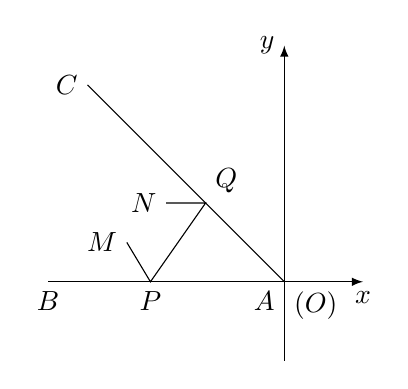
\begin{tikzpicture}[>=latex]
        \draw [->] (-3,0) -- (1,0) node [below] {$x$};
        \draw [->] (0,-1) -- (0,3) node [left] {$y$};
        \draw (0,0) node [below right] {$(O)$};
        \draw (0,0) node [below left] {$A$};
        \draw (-2,0.5) node [left] {$M$} (-1.5,1) node [left] {$N$};
        \draw (-2.5,2.5) node [left] {$C$} -- (0,0);
        \draw (-3,0) node [below] {$B$};
        \draw (-1.5,1) -- (-1,1) node [above right] {$Q$} -- (-1.7,0) node [below] {$P$} -- (-2,0.5);
    \end{tikzpicture}
\end{center}
\item 已知直线$l$: $f(x,y)=0$.如果直线$l$外一点$P$的坐标为$(x_0,y_0)$, 那么直线$f(x,y)$ $-f(x_0,y_0)=0$\bracket{20}.
\twoch{过点$P$且与直线$l$斜交}{过点$P$且与直线$l$重合}{过点$P$且与直线$l$平行}{过点$P$且与直线$l$垂直}
\item 如果直线$x\cos \theta +y-2=0(\theta \in \mathbf{R})$的倾斜角为$\alpha$, 那么$\alpha$的取值范围是\blank{50}.
\item 若直线$l_1$: $a_1x+b_1y+2=0$(实数$a_1,b_1$不同时为$0$)与直线$l_2$: $a_2x+b_2y+2=0$(实数$a_2,b_2$不同时为$0$)的交点为$(1,2)$, 则经过$P(a_1,b_1),Q(a_2,b_2)$两点的直线的方程为\blank{50}.
\item 如果直线$l$经过点$(3,4)$, 且点$(-3,2)$到直线$l$的距离最大, 求这条直线的方程.
\item 已知$\triangle ABC$的三个顶点的坐标分别为$A(2,3)$、$B(4,-1)$、$C(-4,1)$, 直线$l$平行于$AB$, 且将$\triangle ABC$分成面积相等的两部分, 求直线$l$的方程.
\item 过点$P(2,1)$作直线$l$, 分别交$x$轴、$y$轴的正半轴于$AB$两点.当$\triangle AOB$的面积最小时, 求直线$l$的方程.
\item 已知直线$l$经过点$P(1,2)$, 且与两坐标轴围成的三角形面积为$S$.\\
(1) 当$S=3$时, 满足条件的直线有几条?\\
(2) 当$S=4$时, 满足条件的直线有几条?\\
(3) 当$S=5$时, 满足条件的直线有几条?
\item 下列各组方程中表示相同曲线的是\bracket{20}.
\fourch{$y=x$, $\dfrac yx=1$}{$y=x$, $y=\sqrt {x^{2}}$}{$|x|=|y|$, $\sqrt x=\sqrt y$}{$|x|=|y|$, $x^2=y^2$}
\item 方程$y=-\sqrt {x^2-2x+1}$的图形是下图中的\bracket{20}.
\fourch{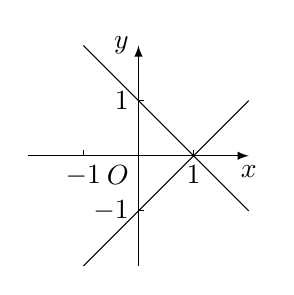
\begin{tikzpicture}[>=latex,scale = 0.7]
    \draw [->] (-2,0) -- (2,0) node [below] {$x$};
    \draw [->] (0,-2) -- (0,2) node [left] {$y$};
    \draw (0,0) node [below left] {$O$};
    \draw (-1,0.1) -- (-1,0) node [below] {$-1$};
    \draw (1,0.1) -- (1,0) node [below] {$1$};
    \draw (0.1,-1) -- (0,-1) node [left] {$-1$};
    \draw (0.1,1) -- (0,1) node [left] {$1$};
    \draw (-1,2) -- (2,-1) (-1,-2) -- (2,1);
\end{tikzpicture}}{\begin{tikzpicture}[>=latex,scale = 0.7]
    \draw [->] (-2,0) -- (2,0) node [below] {$x$};
    \draw [->] (0,-2) -- (0,2) node [left] {$y$};
    \draw (0,0) node [below left] {$O$};
    \draw (-1,0.1) -- (-1,0) node [below] {$-1$};
    \draw (1,0.1) -- (1,0) node [below] {$1$};
    \draw (0.1,-1) -- (0,-1) node [left] {$-1$};
    \draw (0.1,1) -- (0,1) node [left] {$1$};
    \draw (1,0) -- (2,-1) (1,0) -- (2,1);
\end{tikzpicture}}{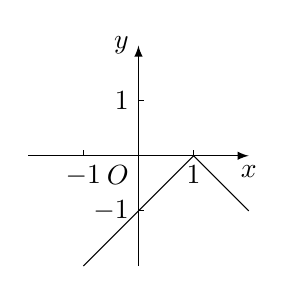
\begin{tikzpicture}[>=latex,scale = 0.7]
    \draw [->] (-2,0) -- (2,0) node [below] {$x$};
    \draw [->] (0,-2) -- (0,2) node [left] {$y$};
    \draw (0,0) node [below left] {$O$};
    \draw (-1,0.1) -- (-1,0) node [below] {$-1$};
    \draw (1,0.1) -- (1,0) node [below] {$1$};
    \draw (0.1,-1) -- (0,-1) node [left] {$-1$};
    \draw (0.1,1) -- (0,1) node [left] {$1$};
    \draw (-1,-2) -- (1,0) (1,0) -- (2,-1);
\end{tikzpicture}}
{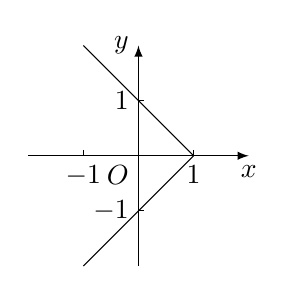
\begin{tikzpicture}[>=latex,scale = 0.7]
    \draw [->] (-2,0) -- (2,0) node [below] {$x$};
    \draw [->] (0,-2) -- (0,2) node [left] {$y$};
    \draw (0,0) node [below left] {$O$};
    \draw (-1,0.1) -- (-1,0) node [below] {$-1$};
    \draw (1,0.1) -- (1,0) node [below] {$1$};
    \draw (0.1,-1) -- (0,-1) node [left] {$-1$};
    \draw (0.1,1) -- (0,1) node [left] {$1$};
    \draw (-1,2) -- (1,0) (-1,-2) -- (1,0);
\end{tikzpicture}}
\item 到原点的距离等于$3$的动点的轨迹方程是$y=\sqrt {9-x^2}$吗? 为什么?
\item 已知点$P(2,1)$在方程$x^2+k^2y^2-3x-ky-4=0$的曲线上, 求实数$k$的值.
\item 定长为$4$的线段$AB$的两端点分别在$x$轴、$y$轴上滑动, 求$AB$中点的轨迹方程.
\item 已知$AB$两点的坐标是$(1,0)$、$(-1,0)$, 动点$M$满足$MA\perp MB$, 求动点$M$的轨迹方程.
\item 已知动点$C$到点$A(2,0)$的距离是它到点$B(8,0)$的距离的一半, 求点$C$的轨迹方程.
\item 已知等腰三角形底边的两个端点的坐标分别是$B(4,2)$、$C(-2,0)$, 求第三个顶点$A$的轨迹方程.
\item 已知曲线$C_1$的方程是$x^2+y^2-4x+3=0$, 曲线$C_2$的方程是$y^2+2x-2=0$, 求这两条曲线的交点.
\item 已知方程$y=k(x-2)$和$x^2+y^2=1$.当实数$k$为何值时, 两方程表示的曲线有两个交点? 只有一个交点? 没有交点?
\item 已知直线$y=ax-1$与曲线$y^2=2x$只有一个交点, 求实数$a$的值.
\item 已知直线$l$: $y=x+b$被曲线$y=\dfrac 12x^2$截得的弦长为$4\sqrt 2$, 求实数$b$的值.
\item 画出下列方程的曲线的图像.\\
(1) $x^2-y^2=0$;\\ 
(2) $x^2+2xy-3y^2=0$.
\item 已知$A(-3,2)$、$B(3,-2)$两点, 求证: 与这两点距离相等的点$M$的轨迹方程是$3x-2y=0$.
\item 已知动点$P$到点$F(4,0)$的距离与它到点$F(-4,0)$的距离的比为$2$, 求点$P$的轨迹方程.
\item 已知曲线$C$: $y^2=x+1$和定点$A(3,1)$, $B$为曲线$C$上任意一点, 若$\overrightarrow {AP}=2\overrightarrow {PB}$, 当点$B$在曲线$C$上运动时, 求点$P$的轨迹方程.
\item 已知直线$y=kx+\dfrac 32$与曲线$y^2-2y-x+3=0$只有一个交点, 求实数$k$的值.
\item 已知直线$l$: $y=x+b$被曲线$C$: $x^2+y^2=9$所截得的线段的长不小于$2$, 求实数$b$的取值范围.
\item 分别根据下列条件, 求相应圆的方程.\\
(1) 圆心为$C(-\dfrac 32,3)$, 半径为$R=\sqrt 3$;\\
(2) 圆心为$C(\sqrt 2,1)$, 过点$A(-1,\sqrt 2)$;\\
(3) 与$x$轴相交于$A(1,0)$、$B(5,0)$两点, 且半径等于$\sqrt 5$.
\item 已知圆$(x-a)^2+(y-b)^2=r^2(r>0)$. 求在下列情况下, 实数$a,b,r$分别应满足什么条件.
(1) 圆过原点;\\
(2) 圆心在$x$轴上;\\
(3) 圆与$x$轴相切;\\
(4) 圆与坐标轴相切.
\item 求经过点$(5,-5)$且与圆$(x-1)^2+(y+2)^2=25$相切的直线的方程.
\item 已知$AB$两点相距$10$厘米, 动点$P$到点$A$的距离是它到点$B$的距离的$3$倍, 求点$P$的轨迹.
\item ``$A=C\ne 0$且$B=0$''是``$Ax^2+Bxy+Cy^2+Dx+Ey+F=0$表示圆的方程''的\blank{50}条件.
\item 直线$Ax+By=0$与圆$x^2+y^2+Ax+By=0$的位置关系是\blank{50}.
\item 已知$a^2x^2+(a+2)y^2+2ax+a=0$表示圆, 求实数$a$的值.
\item 已知圆过原点, 且与$x$轴、$y$轴的交点的坐标分别为$(a,0)$、$(0,b)$, 求这个圆的方程.
\item 求经过点$(5,-5)$且与圆$x^2+y^2=25$相切的直线的方程.
\item 已知动直线$kx-y+1=0$和圆$x^2+y^2=1$相交于$AB$两点, 求弦$AB$的中点的轨迹方程.
\item 已知直线$x\cdot \sin \alpha +y\cdot \cos \alpha +m=0(\alpha \in (0,\dfrac{\pi }2))$被圆$x^2+y^2=2$所截得的线段的长为$\dfrac 43\sqrt 3$, 求实数$m$的值.
\item 已知直线$l$与直线$4x-3y+18=0$垂直, 且它被圆$x^2+y^2-2x+4y-20=0$所截得的线段的长为$8$, 求直线$l$的方程.
\item 求与圆$x^2+y^2=25$外切于点$P(4,-3)$, 且半径为$1$的圆的方程.
\item 已知直线$y=x+m$和曲线$y=\sqrt {1-x^2}$有两个交点, 求实数$m$的取值范围.
\item 求过点$(2,-1)$, 圆心在直线$2x+y=0$上, 且与直线$x-y-1=0$相切的圆的方程.
\item 已知圆$x^2+y^2+6x-8y+25=r^2$与$x$轴相切, 求这个圆截$y$轴所得的弦长.
\item 已知圆$x^2+y^2-2x+2y-3=0$和圆$x^2+y^2+4x-1=0$关于直线$l$对称, 求直线$l$的方程.
\item 已知定点$A(3,1)$, 动点$B$在圆$x^2+y^2=4$上, $P$在线段$AB$上, 且$BP:PA=1:2$, 求点$P$的轨迹方程.
\item 已知圆$C$与$y$轴相切, 圆心点$C$在直线$x-3y=0$上, 且直线$y=x$被圆$C$所截得的线段的长为$2\sqrt 7$, 求圆$C$的方程.
\item 写出分别满足下列条件的椭圆的标准方程.\\
(1) 焦点坐标为$(-6,0)$、$(6,0)$, 且椭圆经过点$(0,8)$;\\
(2) 椭圆经过$(0,-2)$、$(\sqrt 6,0)$两点;\\
(3) 焦距等于$4$, 且椭圆经过点$P(\dfrac{2\sqrt 6}3,-\dfrac{2\sqrt 6}3)$.
\item 已知动点$M$到定点$A(-\dfrac 94,0)$与$B(\dfrac 94,0)$的距离的和是$\dfrac{25}2$, 求点$M$的轨迹方程.
\item 若方程$\dfrac{x^2}m+\dfrac{y^2}{{m^2}-2}=1$表示椭圆, 求实数$m$的取值范围.
\item 若椭圆$\dfrac{x^2}{25}+\dfrac{y^2}9=1$的两个焦点分别为$F_1F_2$, 点$P$为此椭圆上的任意一点, 求$\triangle PF_1F_2$的周长.
\item 已知椭圆的方程为$\dfrac{x^2}{16}+\dfrac{y^2}{m^2}=1(m>0)$.如果此椭圆的焦点在$x$轴上, 那么它的焦距为\bracket{20}.
\fourch{$2\sqrt {16-m^2}$}{$2\sqrt {4-m}$}{$2\sqrt {m^2-8}$}{$2\sqrt {m-4}$}
\item 若方程$16x^2+ky^2=16k$表示焦点在$y$轴上的椭圆, 则实数$k$满足\bracket{20}.
\fourch{$k>16$}{$k=16$}{$k<16$}{$0<k<16$}
\item 已知椭圆$C$的两个焦点分别为$F_1(-3,0)$、$F_2(3,0)$.再添加什么条件, 可得椭圆$C$的方程为$\dfrac{x^2}{25}+\dfrac{y^2}{16}=1$?
\item 求经过$(-\dfrac 32,\dfrac 52)$与$(\sqrt 3,\sqrt 5)$两点的椭圆的标准方程.
\item 若椭圆的方程为$16x^2+25y^2=400$, 则此椭圆的长半轴长为\blank{50}, 短轴长为\blank{50}, 焦距为\blank{50}.
\item 已知椭圆的对称轴为坐标轴.若两个顶点的坐标分别为$(0,13)$、$(-12,0)$, 则此椭圆的焦点坐标为\blank{50}.
\item 若点$(4,3)$在椭圆$\dfrac{x^2}{a^2}+\dfrac{y^2}{b^2}=1(a>b>0)$上, 则\bracket{20}.
\twoch{点$(4,-3)$不在椭圆上}{点$(3,4)$在椭圆上}{点$(-4,-3)$不在椭圆上}{点$(-4,3)$在椭圆上}
\item 过点$(3,-2)$且与椭圆$4x^2+9y^2=36$有相同焦点的椭圆的标准方程是\bracket{20}.
\fourch{$\dfrac{x^2}{15}+\dfrac{y^2}{10}=1$}{$\dfrac{x^2}{{{15}^2}}+\dfrac{y^2}{{{10}^2}}=1$}{$\dfrac{x^2}{10}+\dfrac{y^2}{15}=1$}{$\dfrac{x^2}{{{10}^2}}+\dfrac{y^2}{{{15}^2}}=1$}
\item 若椭圆$\dfrac{x^2}9+\dfrac{y^2}4=1$的弦$AB$被点$P(1,1)$平分, 则$AB$所在直线的方程为 \bracket{20}.
\fourch{$9x+4y-13=0$}{$4x+9y-13=0$}{$x+2y-3=0$}{$x+3y-3=0$}
\item 画出长轴长和短轴长分别为$2$厘米、$1.5$厘米的椭圆的草图.若要把一个边长分别为$2$米和$1.5$米的矩形木板锯成椭圆形, 使它的长轴长和短轴长分别为$2$米、$1.5$米, 请用简便的方法在木板上画出这个椭圆的草图.
\item 已知椭圆以原点为中心, 长轴长是短轴长的$2$倍, 且过点$(-2,-4)$, 求此椭圆的标准方程.
\item $\triangle ABC$的两个顶点$AB$的坐标分别是$(-6,0)$、$(6,0)$, $AC,BC$边所在直线的斜率之积等于$-\dfrac 49$, 求顶点$C$的轨迹方程.
\item 已知椭圆的一个顶点和一个焦点分别是直线$x+3y-6=0$与两坐标轴的交点, 求此椭圆的标准方程.
\item 已知椭圆$C$的焦点分别为$F_1(-2\sqrt 2,0)$、$F_2(2\sqrt 2,0)$, 长轴长为$6$, 直线$y=x+2$交椭圆$C$于$AB$两点, 求线段$AB$的中点的坐标.
\item 已知点$P$是椭圆$\dfrac{x^2}{100}+\dfrac{y^2}{36}=1$上一点, 它到椭圆的左焦点$F_1$的距离是它到右焦点$F_2$的距离的$3$倍.\\
(1) 分别求点$P$与点$F_1$、点$P$与点$F_2$的距离;\\
(2) 求点$P$的坐标.
\item 以椭圆$\dfrac{x^2}{25}+\dfrac{y^2}{16}=1$的两个焦点及短轴的两个端点为四个顶点的椭圆方程为\blank{50}.
\item 如果点$P$是椭圆$\dfrac{x^2}{36}+\dfrac{y^2}{20}=1$上一个动点, $F_1$是椭圆的左焦点, 那么$|PF_1|$的最大值是\blank{50}, $|PF_1|$的最小值是\blank{50}.
\item 如果直线$y=kx+1$与椭圆$\dfrac{x^2}5+\dfrac{y^2}m=1$恒有公共点, 那么实数$m$的取值范围为\blank{50}.
\item 椭圆$\dfrac{x^2}{25}+\dfrac{y^2}9=1$与$\dfrac{x^2}{9-k}+\dfrac{y^2}{25-k}=1(0<k<9)$的关系是\bracket{20}.
\fourch{有相等的长轴和短轴}{有相等的焦距}{有相同的焦点}{有相同的顶点}
\item 在$\triangle ABC$中, 已知$A(-1,0)$、$C(1,0)$.若$a>b>c$, 且满足$2\sin B=\sin A+\sin C$, 则顶点$B$的轨迹的方程是\bracket{20}.
\fourch{$\dfrac{x^2}4+\dfrac{y^2}3=1(x<0)$}{$\dfrac{x^2}3+\dfrac{y^2}4=1(x<0)$}{$\dfrac{x^2}4+\dfrac{y^2}3=1(x>0)$}{$\dfrac{x^2}3+\dfrac{y^2}4=1(x>0)$}
\item 已知椭圆的中心在坐标原点, 它在$x$轴上的一个焦点$F$与短轴$B_1B_2$两端点的连线互相垂直, 且点$F$和长轴上较近的端点$A$的距离是$\sqrt {10}-\sqrt 5$, 求此椭圆的方程.
\item 已知动圆$C$过定点$A(-3,0)$, 且在定圆$B$: $(x-3)^2+y^2=64$的内部与定圆$B$相切, 求动圆的圆心$C$的轨迹方程.
\item 已知椭圆$\dfrac{x^2}{a^2}+\dfrac{y^2}{b^2}=1(a>b>0)$与直线$x+2y-2=0$交于$AB$两点, $|AB|=\sqrt 5$, 且$AB$的中点的坐标为$(m,\dfrac 12)$, 求此椭圆的方程.
\item 写出分别满足下列条件的双曲线的标准方程.\\
(1) 曲线上的点$P$到点$F_1(4,0)$的距离与它到点$F_2(-4,0)$的距离的差的绝对值等于$6$;\\
(2) 曲线上的点$P$到点$F_1(-10,0)$的距离与它到点$F_2(10,0)$的距离的差等于$16$;\\
(3) 焦点在$x$轴上, 且双曲线经过点$(-\sqrt 2,-\sqrt 3)$、$(\dfrac{\sqrt {15}}3,\sqrt 2)$.
\item 设方程$\dfrac{x^2}{m+2}-\dfrac{y^2}{m+1}=1$表示焦点在$y$轴上的双曲线, 求实数$m$的取值范围.
\item 已知双曲线的对称轴为坐标轴, 焦点为$(-6,0)$、$(6,0)$, 且双曲线经过点$(-5,2)$, 求此双曲线的标准方程.
\item 过双曲线$\dfrac{x^2}{16}-\dfrac{y^2}9=1$的右焦点$F_2$作$x$轴的垂线, 求此垂线与双曲线的交点$M$到左焦点$F_1$的距离.
\item 已知双曲线关于原点对称, 它的焦点在坐标轴上, 焦距为$10$, 且此双曲线经过点$(3,4\sqrt 2)$, 求它的标准方程.
\item 已知双曲线$\dfrac{x^2}{64}-\dfrac{y^2}{36}=1$的左、右焦点分别为$F_1,F_2$, 直线$l$过点$F_1$, 交双曲线的左支于$A,B$两点, 且$|AB|=m$, 求$\triangle ABF_2$的周长.
\item 如果中心在原点, 对称轴在坐标轴上的等轴双曲线的一个焦点为$F_1(0,-6)$, 那么此双曲线的标准方程是\blank{50}.
\item 双曲线$2x^2-y^2=8$的焦点坐标是\blank{50}, 两条渐近线的夹角为\blank{50}.
\item 若双曲线的中心在坐标原点, 它的一个焦点的坐标是$(-5,0)$, 两个顶点间的距离为$6$, 则此双曲线的方程是\bracket{20}.
\fourch{$\dfrac{x^2}9-\dfrac{y^2}{16}=1$}{$\dfrac{x^2}{36}-\dfrac{y^2}{11}=1$}{$\dfrac{x^2}{16}-\dfrac{y^2}9=1$}{$\dfrac{x^2}{11}-\dfrac{y^2}{36}=1$}
\item 在下列双曲线中, 以$y=\pm \dfrac 12x$为渐近线的是\bracket{20}.
\fourch{$\dfrac{x^2}{16}-\dfrac{y^2}4=1$}{$\dfrac{x^2}4-\dfrac{y^2}{16}=1$}{$\dfrac{x^2}2-y^2=1$}{$x^2-\dfrac{y^2}2=1$}
\item 若方程$4x^2+ky^2=4k$表示双曲线, 则此双曲线的虚轴长等于\bracket{20}.
\fourch{$2\sqrt k$}{$2\sqrt {-k}$}{$\sqrt k$}{$\sqrt {-k}$}
\item 已知$\triangle ABC$中的两个顶点是$B(0,6)$、$C(0,-6)$, $AB$边与$AC$边所在直线的斜率之积是$\dfrac 49$, 求顶点$A$的轨迹方程.
\item 已知双曲线的虚轴的长为$6$, 一条渐近线的方程为$3x-y=0$, 求此双曲线的标准方程.
\item 求与双曲线$x^2-\dfrac{y^2}4=1$有共同渐近线, 且过点$M(2,2)$的双曲线的标准方程.
\item 已知双曲线$\dfrac{x^2}8-\dfrac{y^2}{b^2}=1$的右焦点为点$F$, 若直线$x-y-3=0$经过点$F$, 求此双曲线渐近线的方程.
\item 已知双曲线$\dfrac{x^2}9-\dfrac{y^2}{16}=1$的两个焦点分别为$F_1F_2$, 点$P$为此双曲线上一点, $|PF_1|\cdot|PF_2|=32$, 求证: $PF_1\perp PF_2$.
\item 求以椭圆$\dfrac{x^2}8+\dfrac{y^2}5=1$的焦点为顶点, 以椭圆的顶点为焦点的双曲线的方程.
\item 已知定点$A(3,0)$和定圆$B$: $(x+3)^2+y^2=16$, 动圆$C$与圆$B$外切, 且过点$A$, 求动圆的圆心$C$的轨迹方程.
\item 已知在$\triangle ABC$中, $A$为动点, $B,C$两定点的坐标分别为$(-2,0),(2,0)$, 且满足$\sin C-\sin B=\dfrac 12\sin A$, 求动点$A$的轨迹方程.
\item 已知直线$l$: $y=ax+1$与双曲线$C$: $3x^2-y^2=1$相交于$AB$两点.\\
(1) 求实数$a$的取值范围;\\
(2) 求当实数$a$为何值时, 以线段$AB$为直径的圆经过坐标原点.
\item 写出分别满足下列条件的抛物线的标准方程.\\
(1) 焦点是$F(1,0)$;\\
(2) 准线方程是$x=-2$.
\item 在抛物线$y^2=20x$上求一点$P$, 使点$P$与焦点的距离等于$15$.
\item 求抛物线$y^2=x$的一组斜率为$2$的平行弦的中点的轨迹方程.
\item 抛物线$y^2=2x$上的$AB$两点到焦点$F$的距离之和是$5$, 求线段$AB$的中点的横坐标.
\item 求抛物线$x=ay^2(a>0)$的焦点坐标与准线方程.
\item 过抛物线$y^2=2px(p>0)$的焦点的一条直线与抛物线相交于两个不同的点, 两个交点的纵坐标分别为$y_1,y_2$, 求证: $y_1y_2=-p^2$.
\item 抛物线$x^2=-32y$的焦点坐标是\blank{50}, 准线方程是\blank{50}.
\item 已知抛物线的顶点在原点, 对称轴为$x$轴, 且过点$(-2,3)$, 求此抛物线的标准方程.
\item 已知抛物线$y^2=8x$的焦点为$F$, $P$在此抛物线上, 且$|PF|=5$, 求点$P$的坐标.
\item 已知一隧道的顶部是抛物拱形, 拱高是$1$米, 跨度为$2$米, 建立适当的直角坐标系, 求相应坐标系下此拱形的抛物线方程.
\item 已知直线$l$: $y=kx-4$与抛物线$y^2=8x$有且只有一个公共点, 求实数$k$的值.
\item 已知正三角形$ABC$的顶点$A$位于坐标原点, 顶点$B$与$C$均在抛物线$y^2=2x$上, 求$\triangle ABC$的边长.
\item 已知直线$l$垂直于$x$轴, 且交抛物线$y^2=4x$于点$AB$, 且$|AB|=4\sqrt 3$, 求直线$AB$的方程.
\item 在抛物线$x^2=\dfrac 14y$上求一点$M$, 使点$M$到直线$y=4x-5$的距离最短.
\item 过点$Q(4,1)$作抛物线$y^2=8x$的弦$AB$, $AB$恰好被点$Q$平分, 求$AB$所在直线的方程.
\item 已知过抛物线$y^2=4x$的焦点$F$的直线交抛物线于$AB$两点, 过原点$O$作$\overrightarrow {OM}$, 使$\overrightarrow {OM}\perp \overrightarrow {AB}$, 垂足为$M$, 求点$M$的轨迹方程.
\item 抛物线$y^2=8x$的动弦$AB$的长为$16$, 求弦$AB$的中点$M$到$y$轴的最短距离.
\item ``太阳火''(sunfire)是一种利用太阳能的装置, 其截面是抛物线形状, 如图所示.``太阳火''依靠抛物线形状的镜面把反射的太阳光聚焦于抛物线的焦点处的锅炉, 加热产生的蒸汽推动汽轮发电机产生电能.根据图中所注尺寸, 求``太阳火''装置中截面抛物线的方程(其中抛物线截面深$10$英尺, 抛物线开口宽$37$英尺).
\begin{center}
    \begin{tikzpicture}[scale = 0.15,>=latex]
        \draw [domain = -18.5:18.5] plot (\x,{\x*\x/40});
        \filldraw [fill = gray!50, draw = black] (0,10) ellipse (2 and 1);
        \draw (-2,10) -- (2,10);
        \draw [->] (20,7) -- (20,10);
        \draw [->] (20,3) -- (20,0);
        \draw (19.5,0) -- (20.5,0) (19.5,10) -- (20.5,10);
        \draw [dashed] (2,10) -- (19.5,10);
        \draw (20,5) node {$10$英尺};
        \draw [->] (-6,-2) -- (-18.5,-2);
        \draw [->] (6,-2) -- (18.5,-2);
        \draw (0,-2) node {$37$英尺};
        \draw (-18.5,-1.5) -- (-18.5,-2.5) (18.5,-1.5) -- (18.5, -2.5);
        \draw [dashed] (0,0) -- (0,10);
        \draw (-2,10) node [left] {锅炉};
    \end{tikzpicture}
\end{center}
\item 下列四个命题中, 正确的是\bracket{20}.
\onech{到两坐标轴距离相等的点的轨迹方程为$y=x$}{两相交直线$y=\dfrac{\sqrt 3}3x$与$y=\sqrt 3x$的夹角平分线的方程为$y=x$}{$\triangle ABC$的三个顶点的坐标分别为$A(1,1)$、$B(3,1)$、$C(1,3)$, $BC$边上的中线方程为$y=x$}{与两顶点$A(-1,0)$、$B(1,0)$的连线的夹角为$90^{\circ }$的动点的轨迹方程为$x^2+y^2=1$}
\item 直线$x-\sqrt 3y=0$绕原点按逆时针方向旋转$30^{\circ }$后所得的直线与圆$(x-2)^2+y^2=3$的位置关系是\bracket{20}.
\twoch{直线过圆心}{直线与圆相交, 但不过圆心}{直线与圆相切}{直线与圆无公共点}
\item 分别求下列各圆的标准方程.\\
(1) 圆心在直线$y=-x$上, 且过$(2,0)$、$(0,-4)$两点;\\
(2) 圆心在直线$2x+y=0$上, 且与直线$x+y-1=0$相切于点$(2,-1)$.
\item 已知圆$O$的方程是$x^2+y^2=1$, 直线$l$与圆$O$相切.\\
(1) 若直线$l$的斜率等于$1$, 求直线$l$的方程;\\
(2) 若直线$l$在$y$轴上的截距为$\sqrt 2$, 求直线$l$的方程.
\item 已知圆$x^2+y^2+x-6y+m=0$与直线$x+2y-3=0$相交于$PQ$两点, $O$为坐标原点, 若$OP\perp OQ$, 求实数$m$的值.
\item 已知圆$C$的圆心在直线$l_1$: $x-3y=0$上, 圆$C$与$y$轴相切, 且直线$l_2$: $x-y=0$被圆$C$所截得的线段的长为$2\sqrt 7$, 求圆$C$的方程.
\item 已知圆$x^2+y^2+6x-7=0$与抛物线$y^2=2ax$的准线相切, 求实数$a$的值.
\item 已知$F_1,F_2$为椭圆$\dfrac{x^2}{16}+\dfrac{y^2}9=1$的两个焦点, 过点$F_2$的直线交椭圆于$AB$两点, 且$|AB|=5$, 求$|AF_1|+|BF_1|$的值.
\item 已知倾斜角为$\dfrac{\pi }4$的直线交椭圆$\dfrac{x^2}4+y^2=1$于$A,B$两点, 求线段$AB$的中点$P$的轨迹方程.
\item 已知过点$M(-2,0)$的直线$l$与椭圆$x^2+2y^2=2$交于$P_1,P_2$两点, 线段$P_1P_2$的中点为$P$, 设直线$l$的斜率为$k_1(k_1\ne 0)$, 直线$OP$的斜率为$k_2$, 求证: $k_1\cdot k_2$的值为定值.
\item 已知椭圆$\dfrac{x^2}{45}+\dfrac{y^2}{20}=1$的焦点分别是$F_1,F_2$, 过中心$O$作直线与椭圆相交于$A,B$两点, 若要使$\triangle ABF_2$的面积是$20$, 求直线$AB$的方程.
\item 椭圆$x^2+4y^2=4$的长轴上的一个顶点为$A$, 以$A$为直角顶点作一个内接于此椭圆的等腰直角三角形, 求这个三角形的面积.
\item 已知点$P$是双曲线$\dfrac{x^2}4-y^2=1$上任意一点, $O$为原点, 求线段$OP$的中点$Q$的轨迹方程.
\item 已知$F_1F_2$为双曲线$\dfrac{x^2}{a^2}-\dfrac{y^2}{b^2}=1(a>0,b>0)$的两个焦点, 过点$F_2$且垂直于$x$轴的直线交双曲线于点$P$, 且$\angle F_1PF_2=60^{\circ }$, 求此双曲线的渐近线的方程.
\item 过点$B(1,1)$能否作直线$l$, 使它与双曲线$x^2-\dfrac{y^2}2=1$交于$Q_1,Q_2$两点, 且点$B$是线段$Q_1Q_2$的中点? 如果存在, 求此直线的方程; 如果不存在, 请说明理由.
\item 已知抛物线的焦点在$y$轴上, 抛物线上一点$M(a,-4)$到焦点$F$的距离为$5$, 求此抛物线的标准方程及实数$a$的值.
\item 过抛物线$y^2=4x$的焦点作直线交抛物线于$A(x_1,y_1)$、$B(x_2,y_2)$两点, 且$x_1+x_2=6$, 求$|AB|$的值.
\item 已知直线$y=x-2$与抛物线$y^2=ax$相交于$AB$两点, 且$OA\perp OB$, 求实数$a$的值.
\item 已知抛物线的顶点是双曲线$16x^2-9y^2=144$的中心, 它的焦点是双曲线的左顶点, 求此抛物线的方程.
\item 如图, 一位运动员在距篮下$4$米处跳起投篮, 球运行的路线是抛物线, 当球运行的水平距离为$2.5$米时, 达到最大高度为$3.5$米, 然后准确落入篮框, 已知篮框中心到地面的距离为$3.05$米.\\
(1) 建立如图所示的平面直角坐标系, 求抛物线的方程;\\
(2) 该运动员身高为$1.8$米, 在这次跳投中, 球在头顶上方$0.25$米处出手, 问球出手时, 他跳离地面的高度是多少.
\item 设圆的方程是$(x-a)^2+(y+b)^2=a^2+b^2$, 其中$a>0,b>0$, 给出下列三种说法:
\textcircled{1} 该圆的圆心$(a,b)$;
\textcircled{2} 该圆过原点;
\textcircled{3} 该圆与$x$轴相交于两个不同点.
其中\bracket{20}.
\fourch{只有\textcircled{1}与\textcircled{2}正确}{只有\textcircled{1}与\textcircled{3}正确}{只有\textcircled{2}与\textcircled{3}正确}{\textcircled{1}、\textcircled{2}与\textcircled{3}都正确}
\item 若椭圆$\dfrac{x^2}4+\dfrac{y^2}{a^2}=1$与双曲线$\dfrac{x^2}{a^2}-\dfrac{y^2}2=1$有相同的焦点, 则实数$a$为\bracket{20}.
\fourch{1}{$-1$}{$\pm 1$}{不确定}
\item 填若抛物线$y^2=2px(p>0)$上一点$M$到焦点的距离为$a(a>\dfrac p2)$, 则点$M$到准线的距离为\blank{50}, 点$M$的横坐标为\blank{50}.
\item 若双曲线$x^2-y^2=1$的右支上有一点$P$到直线$y=x$的距离为$\sqrt 2$, 则点$P$的坐标为\blank{50}.
\item 命题: 椭圆$\dfrac{x^2}{25}+\dfrac{y^2}9=1$与双曲线$\dfrac{x^2}{11}-\dfrac{y^2}5=1$的焦距相等.试将此命题推广到一般情形, 使已知命题成为推广后命题的一个特例:\blank{50}.
\item 已知圆$x^2+y^2+6x-7=0$与抛物线$x^2=2ay$的准线相切, 求实数$a$的值.
\item 求渐近线方程为$3x\pm 4y=0$, 焦点为椭圆$\dfrac{x^2}{10}+\dfrac{y^2}5=1$的一对顶点的双曲线的方程.
\item 设$F_1,F_2$为椭圆$\dfrac{x^2}9+\dfrac{y^2}4=1$的两个焦点, $P$为椭圆上任意一点, 已知$P,F_1,F_2$是一个直角三角形的三个顶点, 且$|PF_1|>|PF_2|$, 求$\dfrac{|PF_1|}{|PF_2|}$的值.
\item 已知双曲线的渐近线方程为$y=\pm x$, 它的两个焦点都在抛物线$x^2=y+2$上, 求此双曲线的方程.
\item 在直角坐标系中, 一物体经过点$A(0,9)$, 其轨迹方程为$y=ax^2+c(a<0)$, $D=(6,7)$为$x$轴上给定区间.\\
(1) 为使物体落在$D$内, 求实数$a$的取值范围;\\
(2) 若物体运动时还经过点$P(2,8.1)$, 则它能否落在$D$内? 并说明理由.
\item (1) 已知直线$l$: $4x-y-1=0$与抛物线$x^2=2y$交于$A(x_A,y_A)$、$B(x_B,y_B)$两点, 直线$l$与$x$轴相交于点$C(x_C,0)$, 求证: $\dfrac 1{x_A}+\dfrac 1{x_B}=\dfrac 1{x_C}$;\\
(2) 试将第(1)题中的命题加以推广, 使得第(1)题中的命题是推广后得到的命题的特例, 并证明推广后得到的命题正确.
\item 复数的代数形式是\blank{50}.
\item 用集合的关系符号表示复数集$\mathbf{C}$、实数集$\mathbf{R}$、有理数集$\mathbf{Q}$、整数集$\mathbf{Z}$和自然数集$\mathbf{N}$的关系为\blank{50}.
\item 若复数$z=a+b\mathrm{i}(a,b\in \mathbf{R})$是虚数, 则$ab$应满足的条件是\bracket{20}.
\fourch{$a=0,b\ne 0$}{$a\ne 0,b\in \mathbf{R}$}{$a\ne 0,b\ne 0$}{$a\in \mathbf{R},b\ne 0$}
\item 已知复数$z_1=a+b\mathrm{i}(ab\in \mathbf{R})$和复数$z_2=c+d\mathrm{i}(cd\in \mathbf{R})$. ``$a=c$''是``$z_1=z_2$''的\bracket{20}.
\twoch{充分非必要条件}{必要非充分条件}{充要条件}{既非充分又非必要条件}
\item 当实数$m$为何值时, 复数$(m^2-3m-4)+(m^2-5m-6)\mathrm{i}(m\in \mathbf{R})$是实数?
\item 当实数$m$为何值时, 复数$(m^2-3m-4)+(m^2-5m-6)\mathrm{i}(m\in \mathbf{R})$是纯虚数?
\item 当实数$m$为何值时, 复数$(m^2-3m-4)+(m^2-5m-6)\mathrm{i}(m\in \mathbf{R})$是零?
\item 已知复数$(3m+2n-5)+(-m+4n+7)\mathrm{i}$是纯虚数, 复数$(2m-n-1)+(m+n+1)\mathrm{i}$是实数, 求实数$m,n$的值.
\item 已知复数$z=(\dfrac 12x+y)+(5x+\dfrac 23y-16)\mathrm{i}$等于$-4$, 求实数$x,y$的值.
\item 求分别满足下列各等式的实数$x$与$y$的值.\\
(1) $(x+y)-xy\mathrm{i}=-5+24\mathrm{i}$;\\
(2) $2x^2-5x+2+(y^2+y-2)\mathrm{i}=0$.
\item 下列有关复数的描述中, 正确的是\bracket{20}.
\twoch{$\mathrm{i}$是$-1$的一个平方根}{$-2\mathrm{i}<-\mathrm{i}$}{$b\mathrm{i}(b\in \mathbf{R})$表示纯虚数}{若$z=3-4\mathrm{i}$, 则$\mathrm{Re}z=3$, $\mathrm{Im}z=4$}
\item 判断是否存在实数$m$, 使复数$z=m^2+2m-15+\dfrac{{m^2}-5m+6}{{m^2}-25}\mathrm{i}$分别满足下列条件.若存在, 求出$m$的值; 若不存在, 请说明理由.\\
(1) $z$是实数;\\
(2) $z$是虚数;\\
(3) $z$是纯虚数;\\
(4) $z$是零.
\item 已知复数$z=x^2-y^2-7+(x-y-3)\mathrm{i}$等于$-2\mathrm{i}$, 求实数$x,y$的值.
\item 已知$2x+3y+(x^2-y^2)\mathrm{i}=y+2+4\mathrm{i}$, 求实数$x,y$的值.
\item 复数$z=-4+3\mathrm{i}$在复平面$xOy$上所对应的点$Z$在第\blank{50}象限, $|z|=$\blank{50}, $|\overrightarrow{OZ}|$\blank{50}.
\item 判断题: (下列命题中, 是真命题的在横线上填入``$\checkmark$''; 是假命题的在横线上填入``$\times$'')
(1) 表示实数的点都在实轴上, 表示纯虚数的点都在虚轴上.\blank{20};\\
(2) 表示虚数的点都落在四个象限内.\blank{20};\\
(3) 复数的模表示该复数在复平面上所对应的点到原点的距离.\blank{20}.
\item 比较复数$z_1=-5+12\mathrm{i}$与$z_2=-8-7\sqrt 2\mathrm{i}$的模的大小.
\item 求实数$m$取何值时, 复数$z=(m^2-8m+15)+(m^2-5m-14)\mathrm{i}$所对应的点$Z$分别满足下列条件.\\
(1) 点$Z$在实轴上;\\
(2) 点$Z$在虚轴上;\\
(3) 点$Z$在第四象限.
\item 已知复数$z$分别满足下列条件, 复数$z$在复平面上对应点$Z$, 画出点$Z$的集合对应的图形.\\
(1) $|z|=3$;\\ 
(2) $|z|<3$;\\
(3) $2\le|z|\le 5$.
\item 已知复数$(m-1)+(2m-3)\mathrm{i}$的模为$1$, 求实数$m$的值.
\item 已知复数$z$的模为$3$.若$\mathrm{Re}z=2$, 则$z=$\blank{50}.
\item ``$|z_1|=|z_2|$''的一个充分非必要条件是\blank{50}.
\item 已知$\overrightarrow{OA}=(5,-1)$, $\overrightarrow{OB}=(3,2)$, 则$\overrightarrow{AB}$在复平面上所对应的复数是\bracket{20}.
\fourch{$5-\mathrm{i}$}{$3+2\mathrm{i}$}{$2-3\mathrm{i}$}{$-2+3\mathrm{i}$}
\item 在复平面上, 平行于$y$轴的非零向量所对应的复数一定是\bracket{20}.
\fourch{实数}{虚数}{纯虚数}{实数或纯虚数}
\item 已知复数$z_1=1-2a\mathrm{i}$, 复数$z_2=a-1+\mathrm{i}$, 且$|z_1|=|z_2|$, 求实数$a$的值.
\item 已知复数$z=x+y\mathrm{i}(x,y\in \mathbf{R})$在复平面上的对应点在直线$x+2y+4=0$上, 求$|z|$的最小值.
\item 复数$z=a+b\mathrm{i}(ab\in \mathbf{R})$的共轭复数是$\overline  z=$\blank{50}, $z$与$\overline  z$在复平面上所对应的点关于\blank{50}对称.
\item 下列四个命题:
\textcircled{1} 复数$z$与它的共轭复数$\overline  z$不能比较大小, 但它们的模相等;
\textcircled{2} 互为共轭的两个复数的和为实数, 而它们的差为纯虚数;
\textcircled{3} 若复数$z$的共轭复数是$-z$, 则$z$一定是纯虚数;
\textcircled{4} 若复数$z$的共轭复数是它自身, 则$z$一定是实数.
其中正确命题的序号是\blank{50}.
\item 计算:\\
(1) $(\dfrac 14-\dfrac{13}5\mathrm{i})+(\dfrac 23+\dfrac 52\mathrm{i})$;\\
(2) $-1-\mathrm{i}-(2+3\mathrm{i})+4\mathrm{i}$;\\
(3) $-(3-4\mathrm{i})+(2+\mathrm{i})-(1-5\mathrm{i})$;\\
(4) $[(a+b)+(a-b)\mathrm{i}]-[(a-b)-(a+b)\mathrm{i}]$.
\item 在下列各组复数中, 前一个复数对应向量$\overrightarrow{OA}$, 后一个复数对应向量$\overrightarrow{OB}$, 对每一组复数分别求向量$\overrightarrow{AB}$与$\overrightarrow{BA}$所对应的复数, 并求向量$\overrightarrow{OA},\overrightarrow{OB}$及$\overrightarrow{AB}$的模.\\
(1) $2-3\mathrm{i}$, $4+5\mathrm{i}$;\\ 
(2) $\dfrac 12-\dfrac{\sqrt 3}2\mathrm{i}$, $\dfrac{\sqrt 3}2+\dfrac 12\mathrm{i}$.
\item 已知$z_1,z_2$为两个复数.\\
(1) 求证: $\overline z_1+\overline z_2=\overline {z_1+z_2}$;\\
(2) 求证: $\overline z_1-\overline z_2=\overline {z_1-z_2}$.
\item 已知复数$z_1z_2$满足$|z_1|=|\overline  z_2|=1$, 且$z_1+z_2=-\mathrm{i}$, 求$z_1z_2$.
\item 已知复数$z=x+y\mathrm{i}(x,y\in \mathbf{R})$满足$|z-1|=1$, 求复数$z$的模的取值范围.
\item 已知复数$z=x+y\mathrm{i}(x,y\in \mathbf{R})$满足$|z|=1$, 求复数$z-1-\mathrm{i}$的模的取值范围.
\item 已知$|z-2|=|z-2\mathrm{i}|$, 写出复数$z$在复平面上所对应的点$Z$的集合是什么图形.
\item ``复数$z_1z_2$互为共轭''是``$|z_1|=|z_2|$''的\blank{50}条件.
\item 若向量$\overrightarrow {OA}\overrightarrow {AB}$所对应的复数分别为$-1-2\mathrm{i}$、$4-\mathrm{i}$, 则点$B$的坐标为\blank{50}.
\item 求证: 非零复数$z$是纯虚数的充要条件是$z+\overline  z=0$.
\item 已知复数$z$满足$|z|+\overline z=1+2\mathrm{i}$, 求复数$z$.
\item 已知复数$z=\cos \theta +\mathrm{i}\sin \theta (\theta \in \mathbf{R})$, 求$|z+2\mathrm{i}|$的取值范围.
\item 已知复数$z$满足$|z+3-4\mathrm{i}|=2$, 求$|z-1|$的取值范围.
\item 计算:\\
(1) $(4-3\mathrm{i})(3+4\mathrm{i})$;\\ 
(2) $(-2+3\mathrm{i})(5-4\mathrm{i})$;\\
(3) $(\dfrac{\sqrt 2}2-\dfrac{\sqrt 2}2\mathrm{i})^2$;\\ 
(4) $(2-5\mathrm{i})(1+2\mathrm{i})(12+\mathrm{i})$.
\item 计算:\\
(1) $\mathrm{i}+\mathrm{i}^2+\mathrm{i}^3+\cdots +\mathrm{i}^{200}$;\\ 
(2) $(1+\mathrm{i})^{10}-(1-\mathrm{i})^{10}$.
\item 已知复数$z_1$、$z_2$, $z_2\ne 0$.\\
(1) 求证: $\overline {z_1\cdot z_2}=\overline z_1\cdot \overline z_2$;\\
(2) 求证: $\overline {(\dfrac{z_1}{z_2})}=\dfrac{\overline {z_1}}{\overline {z_2}}$.
\item 计算:\\
(1) $\dfrac 2{1-\mathrm{i}}$;\\ 
(2) $\dfrac{7+9\mathrm{i}}{1+2\mathrm{i}}$;\\
(3) $\dfrac{6-5\mathrm{i}}{2+3\mathrm{i}}$;\\ 
(4) $\dfrac{\sqrt 5+\sqrt 3\mathrm{i}}{\sqrt 5-\sqrt 3\mathrm{i}}-\dfrac{\sqrt 3+\sqrt 5\mathrm{i}}{\sqrt 3-\sqrt 5\mathrm{i}}$.
\item 已知$z=1-\mathrm{i}$, 求$\dfrac{z^2-z+1}{z^2+z+1}$的值.
\item 已知实数$x,y$满足$\dfrac x{1-\mathrm{i}}+\dfrac y{1-2\mathrm{i}}=\dfrac 5{1-3\mathrm{i}}$, 求$x,y$的值.
\item 计算:\\
(1) $|3-4\mathrm{i}|^4$;\\ 
(2) $|(1+\mathrm{i})^2(\mathrm{i}-2\sqrt 2)^3|$;\\
(3) $|\dfrac{(\sqrt 5-2\mathrm{i}){{(1+\sqrt 3\mathrm{i})}^2}}{\sqrt {13}+\sqrt {23}\mathrm{i}}|$.
\item 已知复数$z$满足$|z|=1$, 且$z\ne \pm \mathrm{i}$, 求证: $\dfrac{z+{\mathrm{i}}}{z-{\mathrm{i}}}$是纯虚数.
\item 计算:\\
(1) $(\dfrac{1-\mathrm{i}}{1+\mathrm{i}})^3$;\\ 
(2) $\dfrac{-2+2\sqrt 3\mathrm{i}}{{{(\sqrt 3+\mathrm{i})}^2}}$;\\
(3) $\dfrac{1+\mathrm{i}}{2+3\mathrm{i}}+\dfrac{3-2\mathrm{i}}{2-3\mathrm{i}}$;\\ 
(4) $\dfrac{{{(1-2\mathrm{i})}^2}}{3-4\mathrm{i}}-\dfrac{{{(2+\mathrm{i})}^2}}{4-3\mathrm{i}}$.
\item 已知$z_1=5+10\mathrm{i}$, $z_2=3-4\mathrm{i}$, 复数$z$满足$\dfrac 1z=\dfrac 1{z_1}+\dfrac 1{z_2}$, 求$z$.
\item 已知复数$z=\dfrac{(1+\sqrt 3)+(1-\sqrt 3)\mathrm{i}}{4+4\mathrm{i}}$, 求$\overline z$及$\dfrac 1z$.
\item 已知复数$z=\dfrac{m+(3m-1){\mathrm{i}}}{2-{\mathrm{i}}}(m\in \mathbf{R})$的实部与虚部互为相反数, 求$|z|$.
\item 求下列复数的平方根.\\
(1) $8-6\mathrm{i}$;\\ 
(2) $-\dfrac 12+\dfrac{\sqrt 3}2\mathrm{i}$;\\
(3) $5\mathrm{i}$.	
\item 利用$1$的立方根, 求下列实数的立方根:\\
(1) $\dfrac 18$;\\ 
(2) $-27$.
\item 计算$(-\dfrac 12-\dfrac{\sqrt 3}2\mathrm{i})^8$的值.
\item 已知$z^2=5-12\mathrm{i}$, 求$\overline z$.
\item $-1$的平方根是\blank{50}, $-1$的立方根是\blank{50}.
\item 非零实数$a$的立方根是\blank{50}.
\item 已知复数$z_1=\sqrt 3+\mathrm{i}$, $|z_2|=1$, $z_1\cdot z_2^2$是虚部为负数的纯虚数, 求复数$z_2$.
\item 判断题: (下列命题中, 是真命题的在横线上填入``$\checkmark$''; 是假命题的在横线上填入``$\times$'')\\
(1) 在复数范围内, 方程$ax^2+bx+c=0$($a,b,c\in \mathbf{R}$, $a\ne 0$)总有两个根.\blank{20};\\
(2) 若$1+2\mathrm{i}$是方程$x^2+px+q=0$的一个根, 则这个方程的另一个根是$1-2\mathrm{i}$.\blank{20};\\
(3) 若方程$x^2+px+q=0$有两个共轭虚根, 则$pq$均为实数.\blank{20}.
\item 若实系数一元二次方程的一个根是$\dfrac 13+\dfrac{\sqrt 7}3\mathrm{i}$, 则这个方程可以是\blank{50}.
\item 在复数集中解下列一元二次方程:\\
(1) $4x^2+9=0$;\\ 
(2) $x^2-x+1=0$;\\
(3) $x^2+4x+12=0$;\\ 
(4) $2(x^2+4)=5x$.
\item 在复数集中分解因式:\\
(1) $x^2+5y^2$;\\ 
(2) $2x^2-6x+5$.
\item 已知关于$x$的方程$2x^2+bx+c=0$($b,c\in \mathbf{R}$)有一个虚根为$\sqrt 2-\sqrt 3\mathrm{i}$, 求方程的另一个根及$b,c$的值.
\item 已知关于$x$的方程$x^2+kx+3=0(k\in \mathbf{R})$有两个虚根$\alpha$和$\beta$, 且$|\alpha -\beta|=2\sqrt 2$, 求$k$的值.
\item 已知两个数的和等于$4$, 它们的积等于$6$, 求这两个数.
\item 已知关于$x$的方程$x^2+kx+k^2-2k=0(k\in \mathbf{R})$有一个模为$1$的虚根, 求$k$的值.
\item 已知关于$x$的实系数一元二次方程$ax^2+bx+c=0$在复数集中的两个根是$\alpha$和$\beta$, 下列结论中恒成立的是\bracket{20}.
\twoch{$\alpha$和$\beta$互为共轭复数}{$\alpha +\beta =-\dfrac ba$, $\alpha \beta =\dfrac ca$}{$b^2-4ac\ge 0$}{$|\alpha -\beta|=\sqrt {(\alpha +\beta)^2-4\alpha \beta }$}
\item 在复数集中解下列方程:\\
(1) $(x-3)(x-5)+2=0$;\\ 
(2) $x^4-16=0$;\\
(3) $x^3+1=0$;\\ 
(4) $\dfrac 1{x+3}-\dfrac 1x=1$.
\item 在复数集中分解因式:\\
(1) $a^2+2ab+b^2+c^2$;\\ 
(2) $x^4+3x^2-10$.
\item 已知关于$x$的方程$x^2-px+1=0(p\in \mathbf{R})$的两个根为$x_1$和$x_2$, 且$|x_1|+|x_2|=3$, 求$p$的值.
\item 已知关于$x$的方程$x^2+(4+\mathrm{i})x+3+p\mathrm{i}=0(p\in \mathbf{R})$有实数根, 求$p$的值, 并解这个方程.
\item 虚数的平方是\bracket{20}.
\fourch{正实数}{虚数}{负实数}{虚数或负实数}
\item 如果复数$z=(a^2-a-2)+(a^2-3a+2)\mathrm{i}$为纯虚数, 那么实数$a$的值为 \bracket{20}.
\fourch{$-1$或$2$}{$-1$}{$2$}{$1$}
\item 如果$z$是$3+4\mathrm{i}$的共轭复数, 那么$|z|$的值是\bracket{20}.
\fourch{5}{$\sqrt {13}$}{1}{25}
\item 如果向量$\overrightarrow{AB}$对应复数$-3+2\mathrm{i}$, 那么向量$\overrightarrow{BA}$对应的复数为\bracket{20}.
\fourch{$3-2\mathrm{i}$}{$3+2\mathrm{i}$}{$-3+2\mathrm{i}$}{$-3-2\mathrm{i}$}
\item 对于复数$z=a+b\mathrm{i}$($ab$为实数), 有\bracket{20}.
\fourch{$|z^2|>|z|^2$}{$|z^2|=|z|^2$}{$|z^2|<|z|^2$}{$|z|^2=z^2$}
\item 如果$a=\dfrac{(-3-\mathrm{i})^2(2-\mathrm{i})}{(1+2\mathrm{i})^3}$, 那么$|a|=$\blank{50}.
\item 如果$z=\sqrt 2+\mathrm{i}$, 那么$\overline {z^2}=$\blank{50}.
\item 如果复数$z$满足$(1+2\mathrm{i})\overline  z=4+3\mathrm{i}$, 那么$z=$\blank{50}.
\item 如果$z=|1-\mathrm{i}|+\mathrm{i}$, 那么$|z|=$\blank{50}.
\item 在复数集中分解因式: $x^2+16=$\blank{50}.
\item 设$\omega =-\dfrac 12+\dfrac{\sqrt 3}2\mathrm{i}$, 求$(1+\omega)(1+\omega ^2)(1+\omega ^4)(1+\omega ^8)$的值.
\item 计算:\\
(1) $\dfrac{-3+29\mathrm{i}}{1+2\mathrm{i}}$;\\ 
(2) $\dfrac{3+\mathrm{i}}{4-2\mathrm{i}}-\dfrac{7-2\mathrm{i}}{1+\mathrm{i}}$;\\
(3) $\dfrac{{{(1+\mathrm{i})}^4}}{1+2\mathrm{i}}+\dfrac{{{(1-\mathrm{i})}^4}}{1-2\mathrm{i}}$;\\ 
(4) $[(\sqrt 3+1)+(\sqrt 3-1)\mathrm{i}]^2$;\\
(5) $(x-1-\sqrt 2\mathrm{i})(x-1+\sqrt 2\mathrm{i})(x-2+\sqrt 3\mathrm{i})(x-2-\sqrt 3\mathrm{i})$.
\item 在复数集内解下列方程:\\
(1) $x^2-2x+5=0$;\\ 
(2) $3x^2+2x+8=0$.
\item 已知复数$z_1=(2x+1)+\mathrm{i}$, $z_2=y+(2-y)\mathrm{i}$.
(1) 若$z_1=z_2$, 且$x,y\in \mathbf{R}$, 求$z_1$.
(2) 若$z_1=z_2$, 且$x\in \mathbf{R}$, $y$为纯虚数, 求$z_1$.
\item 求$m$取什么实数时, 复数$z=(m^2-2m-3)+(m^2-4m+3)\mathrm{i}$分别满足下列条件.\\
(1) $z$是实数;\\
(2) $z$在复平面上对应的点在第一象限.
\item 已知$\alpha, \beta$是共轭复数, 且$(\alpha +\beta)^2-3\alpha \beta \mathrm{i}=4-6\mathrm{i}$, 求$\alpha,\beta$.
\item 已知$3-\mathrm{i}$是关于$x$的实系数一元二次方程$2x^2+px+q=0$的一个根, 求实数$p,q$的值.
\item 已知复数$z$分别满足下列条件, 写出它在复平面上对应的点$Z$的集合分别是什么图形.\\
(1) $|z-\mathrm{i}|=|z-3|$;\\ 
(2) $|z-1+\mathrm{i}|=|z-\mathrm{i}-3|$;\\
(3) $z\overline z+z+\overline z=0$.
\item 已知集合$A=\{z|z=2a-1+a^2\mathrm{i},\ a\in \mathbf{R}\}$. 当实数$a$变化时, 说明集合$A$中元素在复平面上所对应的点的轨迹表示何种曲线.
\item 已知复数$z$满足$|z|\le \dfrac 12$, 求$|z-\mathrm{i}|$的最大值与最小值.
\item 复数集是实数集的扩充, 因此复数在保留实数的一些性质(如$(a+b)^2=a^2+2ab+b^2$等)的同时, 也使得实数的一些性质(如有序性等)在复数集上不能成立.试写出若干个在实数范围内成立, 而在复数范围内不成立的命题.
\item 如果复平面上正方形的三个顶点所对应的复数分别是$1+2\mathrm{i}$、$-2+\mathrm{i}$、$-1-2\mathrm{i}$, 那么第四个顶点所对应的复数是\bracket{20}.
\fourch{$2+\mathrm{i}$}{$2-\mathrm{i}$}{$-2-\mathrm{i}$}{$-1+2\mathrm{i}$}
\item 在复数范围内, 下列命题正确的是\bracket{20}.
\twoch{若$z$是非零复数, 则$z-\overline z$一定是纯虚数}{若复数$z$满足$z^2=-|z^2|$, 则$z$是纯虚数}{若$z_1^2+z_2^2=0$, 则$z_1=0$且$z_2=0$}{若$z_1,z_2$为两个复数, 则$z_1\overline  z_2+\overline  z_1z_2$一定是实数}
\item $\mathrm{i}^{100}+\dfrac 1{\mathrm{i}^{100}}=$\blank{50}.
\item 若$|3+2k\mathrm{i}|=5$, 则实数$k=$\blank{50}.
\item 若$\dfrac{k+3}{2+7\mathrm{i}}$是实数, 则纯虚数$k=$\blank{50}.
\item 若$m$为实数, 复数$(2m-1)+(-3+4m)\mathrm{i}$所表示的点在第三象限, 则$m$的取值范围是\blank{50}.
\item 已知复数$z_1$满足$(z_1-2)\mathrm{i}=1+\mathrm{i}$, 复数$z_2$的虚部为$2$, 且$z_1z_2$是实数, 求复数$z_2$.
\item 已知复数$z$满足$z+\dfrac 1z\in \mathbf{R}$, 且$|z-2|=2$, 求$z$.
\item 已知复数$z$满足$|z-2|=\sqrt {17}$, 且$|z-3|=4$, 求$z$.
\item 已知复数$z$满足: $|z|=1$且$z\ne \pm \mathrm{i}$, 求证: $\dfrac z{1+z^2}$是实数.
\item 复数等式$|z-z_0|=1$在复平面上表示以$z_0$对应的点为圆心、以$1$为半径的圆.请再写出两个复数等式, 并说明它们在复平面上的几何意义.
\item 若直线$ax+2y+2=0$与直线$3x-y-2=0$平行, 则实数$a=$\blank{50}.
\item 若直线$x-2y-2k=0$与$y=x+k$的交点在圆$x^2+y^2=25$上, 则实数$k=$\blank{50}.
\item 圆的方程为$x^2+y^2+kx+2y+k^2=0$, 当圆的面积最大时, 圆心坐标是\blank{50}.
\item 若点$A(-2,3)$在抛物线$y^2=2px(p>0)$的准线上, 则实数$p$的值为\blank{50}.
\item 集合$\{z|z=\mathrm{i}^n+\dfrac 1{\mathrm{i}^n}, \ n\in \mathbf{N}^*\}$用列举法可表示为\blank{50}.
\item 方程为$2x^2-5xy+2y^2=1$的曲线\bracket{20}.
\twoch{关于$x$轴对称}{关于$y$轴对称}{关于直线$y=x$对称, 也关于直线$y=-x$对称}{关于原点对称, 但不关于直线$y=x$对称}
\item 已知$F_1,F_2$是定点, $|F_1F_2|=6$.若动点$M$满足$|MF_1|+|MF_2|=6$, 则动点$M$的轨迹是\bracket{20}.
\fourch{直线}{线段}{圆}{椭圆}
\item 经过点$P(4,-2)$的抛物线的标准方程是\bracket{20}.
\fourch{$y^2=x$或$x^2=y$}{$y^2=x$或$x^2=8y$}{$x^2=y$或$y^2=-8x$}{$y^2=x$或$x^2=-8y$}
\item 如果实数$x,y$满足$(x-2)^2+y^2=3$, 那么$\dfrac yx$的最大值是\bracket{20}.
\fourch{$\dfrac 12$}{$\dfrac{\sqrt 3}3$}{$\dfrac{\sqrt 3}2$}{$\sqrt 3$}
\item 已知点$A(m,m+1)$与点$B(2,m-1)$, 求直线$AB$的倾斜角$\theta$和斜率$k$.
\item 已知直线$mx+4y-2=0$与$2x-5y+n=0$互相垂直, 垂足为$(1,p)$, 求实数$m,n,p$的值.
\item 已知直线$l_1$通过点$(0,-3)$, 且方向向量为$\overrightarrow d=(1,2)$, 直线$l_2$的方程是$3x+y+2=0$.求这两条直线的夹角$\alpha$的大小.
\item 已知双曲线的中心是坐标原点, 它的一条渐近线方程为$3x-4y=0$, 且此双曲线经过点$(2,1)$, 求此双曲线的标准方程.
\item 已知椭圆$\dfrac 12x^2+y^2=1$和椭圆外一点$(0,2)$, 过这点引直线与椭圆交于$A,B$两点, 求弦$AB$的中点$P$的轨迹方程.
\item 已知双曲线的中心在原点, 且它的一个焦点为$F(\sqrt 7,0)$, 直线$y=x-1$与其相交于$MN$两点, 线段$MN$中点的横坐标为$-\dfrac 23$, 求此双曲线的方程.
\item 直线$x-y+1=0$与椭圆$mx^2+ny^2=1(m,n>0)$相交于$AB$两点, 弦$AB$的中点的横坐标是$-\dfrac 13$.求双曲线$\dfrac{y^2}{m^2}-\dfrac{x^2}{n^2}=1$的两条渐近线所夹锐角的大小.
\item 如图, 双曲线$x^2-\dfrac{y^2}4=1$的左、右两个焦点为$F_1,F_2$, 第二象限内的一点$P$在双曲线上, 且$\angle F_1PF_2=\dfrac{\pi }3$.
\begin{center}
    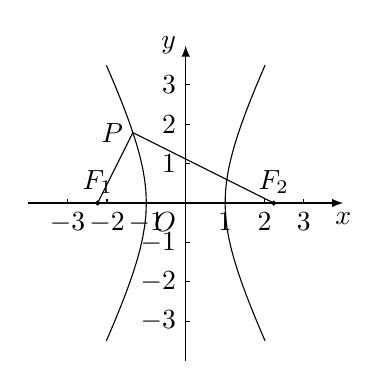
\begin{tikzpicture}[>=latex, scale = 0.5]
        \draw [->] (-4,0) -- (4,0) node [below] {$x$};
        \draw [->] (0,-4) -- (0,4) node [left] {$y$};
        \draw (0,0) node [below left] {$O$};
        \foreach \i in {-3,-2,-1,1,2,3}
        {
          \draw (\i,0.1) -- (\i,0) node [below] {$\i$};
          \draw (0.1,\i) -- (0,\i) node [left] {$\i$};
        };
        \filldraw ({-sqrt(5)},0) circle (0.05) node [above] {$F_1$} coordinate (F1);
        \filldraw ({sqrt(5)},0) circle (0.05) node [above] {$F_2$} coordinate (F2);
        \draw [domain = -3.5:3.5] plot ({sqrt(\x*\x/4+1)},\x);
        \draw [domain = -3.5:3.5] plot ({-sqrt(\x*\x/4+1)},\x);
        \draw ({-3/sqrt(5)},{4/sqrt(5)}) node [left] {$P$} coordinate (P);
        \draw (F1) -- (P) -- (F2);
    \end{tikzpicture}
\end{center}
(1) 求$|PF_1|\cdot|PF_2|$;\\
(2) 求点$P$的坐标.
\item 设复数$z$满足$|z|-\overline  z-5\mathrm{i}-1=0$, 求$z$.
\item 已知复数$z=\log _2(x^2-3x-2)+\mathrm{i}\log _2(x-3)$.\\
(1) 当$x$为何实数时, $z$为实数?\\
(2) 当$x$为何实数时, $z$为纯虚数?\\
(3) 当$x$为何实数时, $z$在复平面上对应的点位于第三象限?
\item 已知虚数$z_1,z_2$满足$z_1^2=z_2$.\\
(1) 设$z_1,z_2$是一个实系数一元二次方程的两个根, 求$z_1,z_2$.\\
(2) 设$z_1=1+m\mathrm{i}$, $m>0$, $|z_1|\le \sqrt 2$, 复数$w=z_2+3$, 求$|w|$的取值范围.
\item 已知$A(-2,-1)$、$B(2,5)$两点.若直线$3x+ay-6=0$过线段$AB$的中点, 则实数$a$的值等于\blank{50}.
\item 点$A$是圆$C$: $x^2+y^2+ax+4y-5=0$上一点.若点$A$关于直线$x+2y-1=0$的对称点也在圆$C$上, 则实数$a=$\blank{50}.
\item 若点$P$在圆$x^2+y^2+4x-6y+12=0$上, 点$Q$在直线$4x+3y-21=0$上, 则$|PQ|$的最小值为\blank{50}.
\item 已知双曲线的中心为原点, 两条渐近线方程是$y=\pm \dfrac 23x$.若这条双曲线过点$M(\dfrac 92,-1)$, 则这条双曲线的焦距为\blank{50}.
\item 若抛物线$x^2=y$上的点到直线$y=2x+b$的最短距离为$\sqrt 5$, 则实数$b=$\blank{50}.
\item 若$\theta \in \mathbf{R}$, 则方程$x^2+y^2\sin \theta =1$所表示的曲线一定不是\bracket{20}.
\fourch{直线}{圆}{抛物线}{双曲线}
\item 若$|z_1|=|z_2|=1$, $|z_1+z_2|=\sqrt 3$, 则$|z_1-z_2|$的值是\bracket{20}.
\fourch{1}{$\sqrt 2$}{$\dfrac{\sqrt 2}2$}{$\dfrac{\sqrt 3}2$}
\item 若复数$z$满足$|z-2\mathrm{i}|^2-|z-1|^2=5$, 则它在复平面中对应的点的轨迹是\bracket{20}.
\fourch{直线}{圆}{双曲线}{椭圆}
\item 已知双曲线的中心在原点, 且它的一个焦点为$F_1(-\sqrt 5,0)$.若点$P$位于此双曲线上, 线段$PF_1$的中点坐标为$(0,2)$, 则此双曲线的方程是\bracket{20}.
\fourch{$\dfrac{x^2}4-\dfrac{y^2}1=1$}{$x^2-\dfrac{y^2}4=1$}{$\dfrac{x^2}2-\dfrac{y^2}3=1$}{$\dfrac{x^2}3-\dfrac{y^2}2=1$}
\item 过点$M(1,2)$作直线交$y$轴于点$B$, 过点$N(-1,-1)$作直线与直线$MB$垂直, 且交$x$轴于点$A$.求线段$AB$的中点的轨迹方程.
\item 在直线$x+3y=0$上求一点, 使它到原点的距离与它到直线$x+3y-2=0$的距离相等.
\item 已知抛物线$y^2=4x$与椭圆$\dfrac{x^2}9+\dfrac{y^2}k=1$有公共焦点$F_1$, 椭圆的另一焦点为$F_2$, $P$是这两条曲线的一个交点, 求$\triangle PF_1F_2$的周长.
\item 已知抛物线$y=2x^2$上有$A(x_1,y_2)$、$B(x_2,y_2)$两点, 且$,B$关于直线$y=x+m$对称, $x_1x_2=-\dfrac 12$, 求实数$m$的值.
\item 设关于$x$的实系数一元二次方程$x^2-ax+b=0$的两个根依次为$\alpha, \beta$, 关于$x$的实系数一元二次方程$x^2+bx+a=0$的两个根依次为$\alpha -1$、$\beta -1$, 求$\alpha, \beta$的值.
\item $A,B,C$是我方三个炮兵阵地, $A$在$B$的正东, 相距$6$千米; $C$在$B$的北偏西$30^{\circ }$, 相距$4$千米.$P$为敌炮兵阵地.某时刻$A$发现$P$地某种信号, 4秒后$BC$两地才同时发现这种信号(该信号的传播速度为$1$千米/秒). 若从$A$地炮击$P$地, 求准确炮击的方位角(精确到$0.1^{\circ }$).
\begin{center}
    \begin{tikzpicture}[>=latex]
        \draw (3,0) node [right] {$A$} -- (0,0) node [below] {$B$} coordinate (B) -- (120:2) node [above] {$C$} coordinate (C);
        \draw [dashed] (0,2) coordinate (y) -- (B);
        \draw [->] (2.5,1) -- (2.5,2) node [right] {北};
        \draw (B) pic ["$30^\circ$",draw, angle eccentricity = 1.9] {angle = y--B--C};
    \end{tikzpicture}
\end{center}
\item 已知直线$l$过点$A(-3,1)$, 且倾斜角为$45^{\circ }$.直线$l$与焦点为$(-\sqrt 6,0)$、$(\sqrt 6,0)$的椭圆交于$B,C$两点, 且点$A$为线段$BC$的中点.是否存在满足上述条件的椭圆? 若存在, 求椭圆的方程; 若不存在, 请说明理由.
\item 如图, 直线$y=\dfrac 12x$与抛物线$y=\dfrac 18x^2-4$交于$AB$两点, 线段$AB$的垂直平分线与直线$y=-5$交于点$Q$.
\begin{center}
    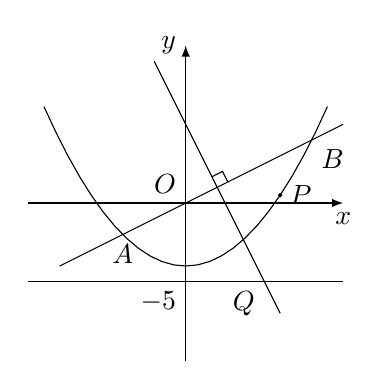
\begin{tikzpicture}[>=latex,scale = 0.2]
        \draw [->] (-10,0) -- (10,0) node [below] {$x$};
        \draw [->] (0,-10) -- (0,10) node [left] {$y$};
        \draw (0,0) node [above left] {$O$};
        \draw [name path = line, domain = -8:10] plot (\x,{\x/2});
        \draw [name path = para, domain = -9:9] plot (\x,{pow(\x,2)/8-4});
        \draw (-10,-5) -- (10,-5);
        \draw (0,-5) node [below left] {$-5$};
        \draw (-4,-2) node [below] {$A$} coordinate (A);
        \draw (8,4) node [below right] {$B$} coordinate (B);
        \filldraw (6,{36/8-4}) circle (0.1) node [right] {$P$};
        \draw (-2,9) coordinate (T) -- (6,-7) (5,-5) node [below left] {$Q$};
        \draw (2,1) coordinate (V);
        \draw (V) pic [draw, scale = 0.3] {right angle = B--V--T};

    \end{tikzpicture}
\end{center}
(1) 求点$Q$的坐标;\\
(2) 当$P$为抛物线上位于线段$AB$下方(含点$AB$)的动点时, 求$\triangle OPQ$面积的最大值.


\end{enumerate}

\end{document}